\documentclass[table]{beamer}
%[]中可以使用draft、handout、screen、transparency、trancompress、compress等参数

%指定beamer的模式与主题
\mode<presentation>
{
  \usetheme{Madrid}
%\usetheme{Boadilla}
%\usecolortheme{default}
%\usecolortheme{orchid}
%\usecolortheme{whale}
%\usefonttheme{professionalfonts}
}

%\usetheme{Madrid}
%这里还可以选择别的主题:Bergen, Boadilla, Madrid, AnnArbor, CambridgeUS, Pittsburgh, Rochester, Warsaw, ...
%有导航栏的Antibes, JuanLesPins, Montpellier, ...
%有内容的Berkeley, PaloAlto, Goettingen, Marburg, Hannover, ...
%有最小导航栏的Berlin, Ilmenau, Dresden, Darmstadt, Frankfurt, Singapore, Szeged, ...
%有章和节表单的Copenhagen, Luebeck, Malmoe, Warsaw, ...

%\usecolortheme{default}
%设置内部颜色主题(这些主题一般改变block里的颜色);这个主题一般选择动物来命名
%这里还可以选择别的颜色主题,如默认的和有特别目的的颜色主题default,structure,sidebartab,全颜色主题albatross,beetle,crane,dove,fly,seagull,wolverine,beaver

%\usecolortheme{orchid}
%设置外部颜色主题(这些主题一般改变title里的颜色);这个主题一般选择植物来命名
%这里还可以选择别的颜色主题,如默认的和有特别目的的颜色主题lily,orchid,rose

%\usecolortheme{whale}
%设置字体主题;这个主题一般选择海洋动物来命名
%这里还可以选择别的颜色主题,如默认的和有特别目的的颜色主题whale,seahorse,dolphin

%\usefonttheme{professionalfonts}
%类似的还可以定义structurebold,structuresmallcapsserif,professionalfonts


% 控制 beamer 的风格,可以根据自己的爱好修改
%\usepackage{beamerthemesplit} %使用 split 风格
%\usepackage{beamerthemeshadow} %使用 shadow 风格
%\usepackage[width=2cm,dark,tab]{beamerthemesidebar}

%插入音标
\usepackage{tipa}
\AtBeginDocument{
  \renewcommand\textipa{\fontencoding{T3}\selectfont}
}
\AtBeginDocument{
  \renewcommand\textipa[2][r]{{\fontfamily{cm#1}\tipaencoding #2}}
}
\renewenvironment{IPA}[1][r]
 {\fontfamily{cm#1}\tipaencoding}
 {}

% 设定英文字体
%\usepackage{fontspec}
\usepackage[no-math]{fontspec}
\setmainfont{Times New Roman}
\setsansfont{Arial}
\setmonofont{Courier New}

% 设定中文字体
\usepackage[BoldFont,SlantFont,CJKchecksingle,CJKnumber]{xeCJK}
%\setCJKmainfont[BoldFont={Adobe Heiti Std},ItalicFont={Adobe Kaiti Std}]{Adobe Song Std}
\setCJKmainfont[BoldFont={Adobe Heiti Std},ItalicFont={Adobe Kaiti Std}]{WenQuanYi Micro Hei}
\setCJKsansfont{Adobe Heiti Std}
\setCJKmonofont{Adobe Fangsong Std}
\punctstyle{hangmobanjiao}

\defaultfontfeatures{Mapping=tex-text}
\usepackage{xunicode}
\usepackage{xltxtra}

\XeTeXlinebreaklocale "zh"
\XeTeXlinebreakskip = 0pt plus 1pt minus 0.1pt

\usepackage{setspace}
\usepackage{colortbl,xcolor}
\usepackage{hyperref}
%\hypersetup{xetex,bookmarksnumbered=true,bookmarksopen=true,pdfborder=1,breaklinks,colorlinks,linkcolor=blue,filecolor=black,urlcolor=cyan,citecolor=green}
\hypersetup{xetex,bookmarksnumbered=true,bookmarksopen=true,pdfborder=1,breaklinks,colorlinks,linkcolor=cyan,filecolor=black,urlcolor=blue,citecolor=green}

% 插入图片
\usepackage{graphicx}
\graphicspath{{figures/}}
% 图文混排
\usepackage{picins}
\usepackage{floatflt}

% 可能用到的包
\usepackage{amsmath,amssymb}
%插入多媒体
%\usepackage{media9}
%\usepackage{movie15}
\usepackage{multimedia}
\usepackage{multicol}
\usepackage{multirow}

% 定义一些自选的模板,包括背景、图标、导航条和页脚等,修改要慎重
% 设置背景渐变由10%的红变成10%的结构颜色
%\beamertemplateshadingbackground{red!10}{structure!10}
%\beamertemplatesolidbackgroundcolor{white!90!blue}
% 使所有隐藏的文本完全透明、动态,而且动态的范围很小
\beamertemplatetransparentcovereddynamic
% 使itemize环境中变成小球,这是一种视觉效果
\beamertemplateballitem
% 为所有已编号的部分设置一个章节目录,并且编号显示成小球
\beamertemplatenumberedballsectiontoc
% 将每一页的要素的要素名设成加粗字体
\beamertemplateboldpartpage

% item逐步显示时,使已经出现的item、正在显示的item、将要出现的item呈现不同颜色
\def\hilite<#1>{
 \temporal<#1>{\color{gray}}{\color{blue}}
    {\color{blue!25}}
}

\renewcommand{\today}{\number\year 年 \number\month 月 \number\day 日}

%五角星
\usepackage{MnSymbol}

%去除图表标题中的figure等
\usepackage{caption}
\captionsetup{labelformat=empty,labelsep=none}

\usepackage{tabu}
\usepackage{multirow}
%表格自动换行
\usepackage{tabularx} 

% 千分号
%\usepackage{textcomp}

%罗马数字
\makeatletter
\newcommand{\rmnum}[1]{\romannumeral #1}
\newcommand{\Rmnum}[1]{\expandafter\@slowromancap\romannumeral #1@}
\makeatother

%分栏
\usepackage{multicol}

%\usepackage{enumitem}
%\usepackage{enumerate}

%键盘
\usepackage{keystroke}

%插入源代码
\usepackage{listings}
\lstset{
  language=bash,                  % 程序语言名称:TeX, Perl, R, sh, bash, Awk
  basicstyle=\normalsize\tt,      %\tt指monospace字体族,程序源代码使用此族字体表示更加美观
  numbers=left,                   % 行号位置(左侧)
  numberstyle=\small,             % 行号字体的字号
  stepnumber=1,                   % 行号的显示步长
  numbersep=5pt,                  % 行号与代码间距
  backgroundcolor=\color{white},  % 背景色;需要 \usepackage{color}
  showspaces=false,               % 不显示空格
  showstringspaces=false,         % 不显示代码字符串中的空格标记
  showtabs=false,                 % 不显示 TAB
  tabsize=4, 
  frame=shadowbox,                % 把代码用带有阴影的框圈起来
  captionpos=b,                   % 标题位置
  breaklines=true,                % 对过长的代码自动断行
  breakatwhitespace=false,        % 断行只在空格处
  extendedchars=false,            % 解决代码跨页时,章节标题,页眉等汉字不显示的问题
  %escapeinside={\%*}{*},         % 跳脱字符,添加注释,暂时离开 listings 
  %escapeinside=``,
  commentstyle=\color{red!50!green!50!blue!50}\tt,  %浅灰色的注释
  rulesepcolor=\color{red!20!green!20!blue!20},     %代码块边框为淡青色
  keywordstyle=\color{blue!70}\bfseries\tt,         %代码关键字的颜色为蓝色,粗体
  identifierstyle=\tt,
  stringstyle=\tt,                % 代码字符串的特殊格式
  keepspaces=true,
  breakindent=1em,
  %breakindent=22pt,
  %breakindent=4em,
  breakautoindent=true,
  flexiblecolumns=true,
  aboveskip=1em,                  %代码块边框
  xleftmargin=2em,
  xrightmargin=2em
}

%\setbeamercolor{alerted text}{fg=magenta}
\setbeamercolor{bgcolor}{fg=yellow,bg=cyan}
%\setbeamercolor{itemize/enumerate body}{fg=green}

\begin{document}

%\includeonlyframes{current}

\logo{
\includegraphics[height=0.08\textwidth]{tijmu.png}}

% 在每个Section前都会加入的Frame
\AtBeginSection[]
{
  \begin{frame}<beamer>
    %\frametitle{Outline}
    \frametitle{教学提纲}
    \setcounter{tocdepth}{3}
    \begin{multicols}{2}
      \tableofcontents[currentsection,currentsubsection]
      %\tableofcontents[currentsection]
    \end{multicols}
  \end{frame}
}
% 在每个Subsection前都会加入的Frame
\AtBeginSubsection[]
{
  \begin{frame}<beamer>
%%\begin{frame}<handout:0>
%% handout:0 表示只在手稿中出现
    \frametitle{教学提纲}
    \setcounter{tocdepth}{3}
    \begin{multicols}{2}
    \tableofcontents[currentsection,currentsubsection]
    \end{multicols}
%% 显示在目录中加亮的当前章节
  \end{frame}
}

% 为当前幻灯片设置背景
%{
%\usebackgroundtemplate{
%\vbox to \paperheight{\vfil\hbox to
%\paperwidth{\hfil
\includegraphics[width=2in]{tijmu_charcoal.png}\hfil}\vfil}
%}
\begin{frame}[plain]
  \begin{center}
    {\Huge Linux系统概论\\}
    \vspace{1cm}
    {\LARGE 天津医科大学\\}
    %\vspace{0.2cm}
    {\LARGE 生物医学工程与技术学院\\}
    \vspace{1cm}
    {\large 2017-2018学年下学期(春)\\ 2016级生信班}
  \end{center}
\end{frame}
%}



%\includeonlyframes{current}

\title[软件安装]{第六章\quad 软件安装}
\author[Yixf]{伊现富(Yi Xianfu)}
\institute[TIJMU]{天津医科大学(TIJMU)\\ 生物医学工程与技术学院}
\date{2018年6月}


\begin{frame}
  \titlepage
\end{frame}

\begin{frame}[plain,label=current]
  \frametitle{教学提纲}
  \setcounter{tocdepth}{3}
  \begin{multicols}{2}
    \tableofcontents
  \end{multicols}
\end{frame}


\section{引言}
\begin{frame}
  \frametitle{引言 | 软件}
  \begin{figure}
    \centering
    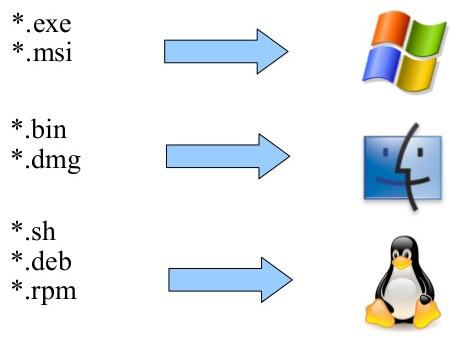
\includegraphics[width=8cm]{c6_software.png}
  \end{figure}
\end{frame}

\begin{frame}
  \frametitle{引言 | 软件 | Windows vs. Linux}
  Windows平台下软件安装的易用性非常不错。多数时候就是一个可执行的exe或msi文件,双击然后一路点击下一步即可;又或者解压后就可以直接运行。基本上,会用电脑的人都知道怎样在Windows上安装软件。\\
  \vspace{5pt}
  软件包包含程序运行的所需文件。但同样是“包”,又可以分两种,一种是源文件包,一种是已经编译过的二进制包。二进制文件计算机可以直接执行,比如Windows下的exe文件,或者Ubuntu下的deb包;而源文件则不行,需要编译才可以。那为什么Linux下软件包不全部以二进制可直接执行的形式提供呢?这是因为Linux系统种类繁多,所使用的二进制有所不同,需要分别打包才行,比如,x86架构跟AMD64的需要分别提供,32位系统与64位的也需要分别提供。\\
  \vspace{5pt}
  也就是说,Windows下提供的软件安装文件基本都是已编译过的,而Linux下就不一定。
\end{frame}

\begin{frame}
  \frametitle{引言 | 软件管理 | 金山卫士软件管理}
  \begin{figure}
    \centering
    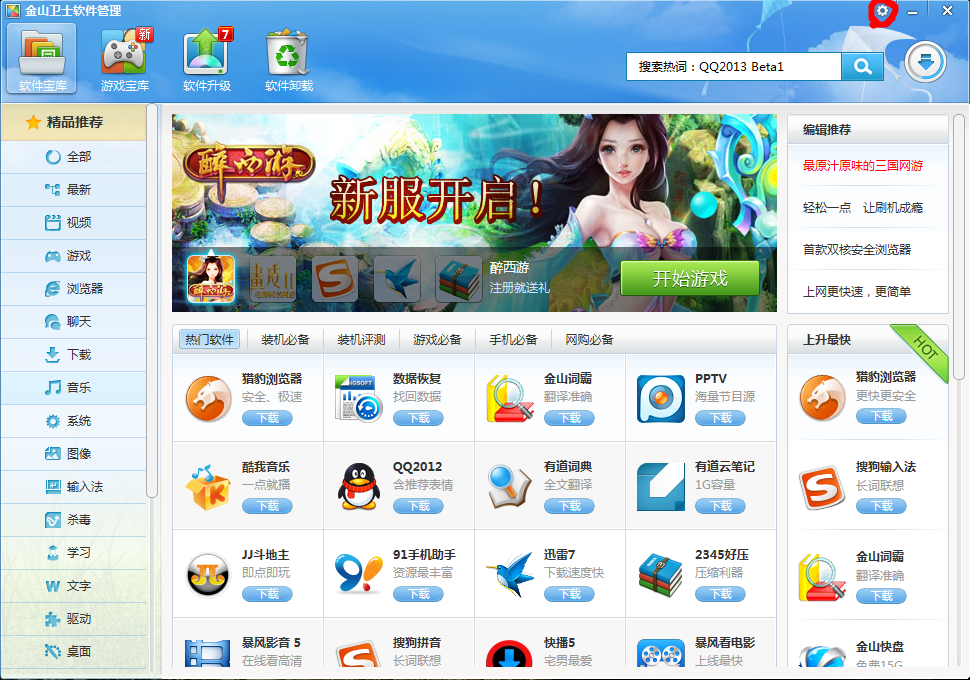
\includegraphics[width=10.5cm]{c6_soft_manager.png}
  \end{figure}
\end{frame}

\begin{frame}
  \frametitle{引言 | 软件管理 | Deepin深度商店}
  \begin{figure}
    \centering
    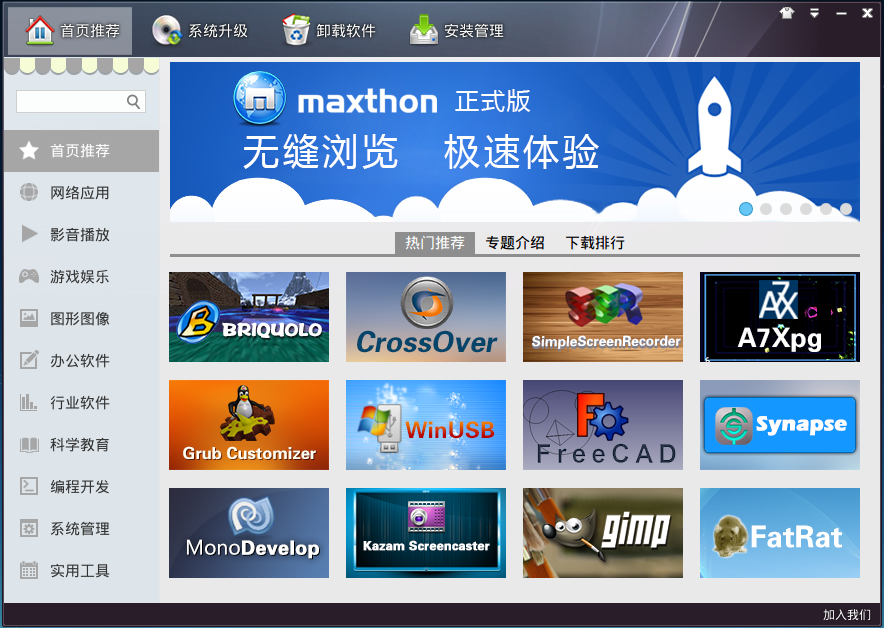
\includegraphics[width=10.5cm]{c6_soft_manager_deepin.png}
  \end{figure}
\end{frame}

\begin{frame}
  \frametitle{引言 | 软件管理 | Ubuntu Kylin软件中心}
  \begin{figure}
    \centering
    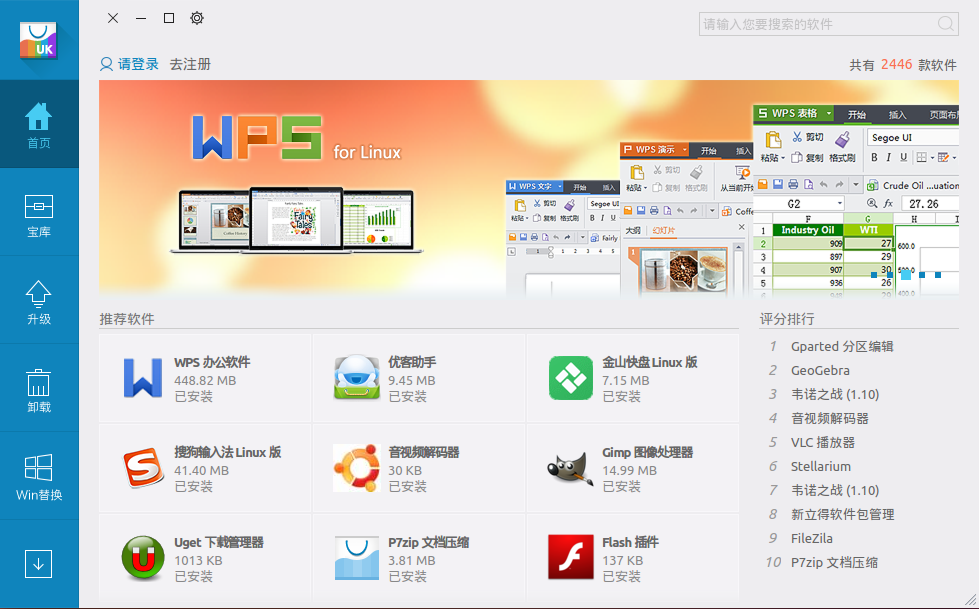
\includegraphics[width=10.5cm]{c6_soft_manager_kylin.png}
  \end{figure}
\end{frame}

\begin{frame}
  \frametitle{引言 | 软件管理 | Ubuntu软件中心}
  \begin{figure}
    \centering
    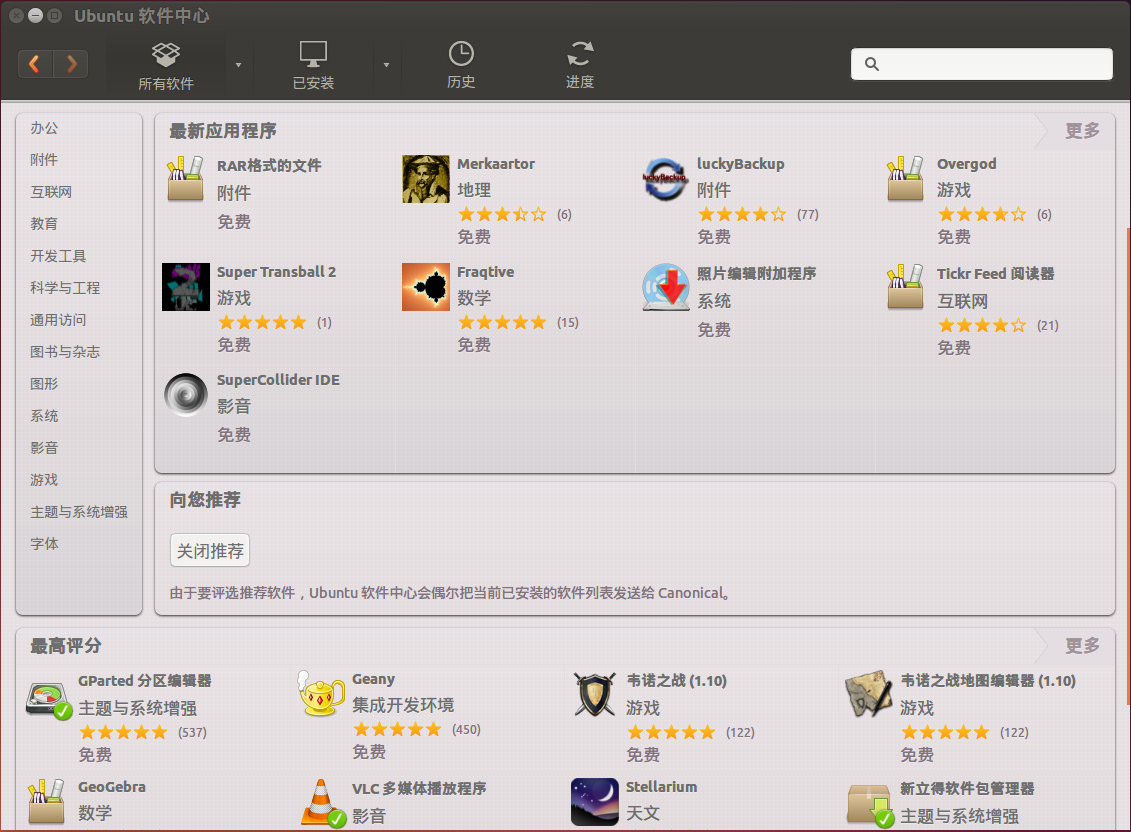
\includegraphics[width=10cm]{c6_soft_center.png}
  \end{figure}
\end{frame}

\begin{frame}
  \frametitle{引言 | 软件管理 | 新立得软件包管理器}
  \begin{figure}
    \centering
    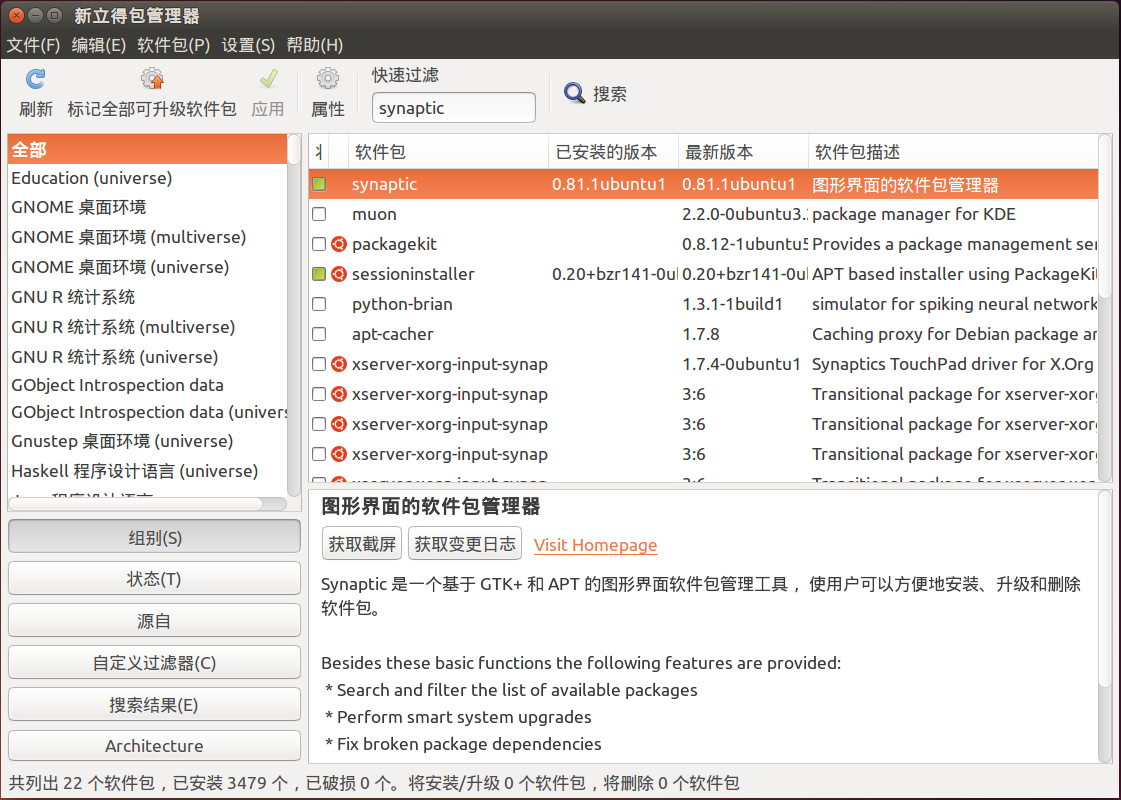
\includegraphics[width=10.5cm]{c6_soft_synaptic.png}
  \end{figure}
\end{frame}

\begin{frame}
  \frametitle{引言 | 软件包管理系统}
  \begin{block}{软件包管理系统}
    Linux软件包管理系统是在电脑中自动安装、配制、卸载和升级软件包的工具组合,在各种系统软件和应用软件的安装管理中均有广泛应用。\\
    使用软件包管理系统将大大简化在Linux发行版中安装软件的过程。
  \end{block}
  \pause
  \begin{block}{\alert{软件包}}
    \begin{itemize}
      \item 二进制包(预编译的软件包)
	\begin{itemize}
    \item deb软件包:Debian, Ubuntu, Linux Mint
	  \item rpm软件包:RHEL, CentOS,Fedora, SUSE, openSUSE, Mandriva Linux, Mageia, PCLinuxOS
	\end{itemize}
      \item 源代码安装包
      \item 脚本安装包
    \end{itemize}
  \end{block}
\end{frame}

\begin{frame}
  \frametitle{引言 | 软件包管理系统}
  \begin{block}{\alert{二进制包管理系统}}
    \begin{description}
      \item[dpkg及其前端APT] Ubuntu, Debian, Linux Mint, Deepin
      \item[RPM及其前端Yum] Red Hat Enterprise Linux, CentOS, Fedora
      \item[ZYpp及其前端Zypper] SUSE, openSUSE
      \item[urpmi] Mandriva Linux, Mageia Linux, ROSA Linux
      \item[pacman] Manjora, Arch Linux
      \item[Portage] Gentoo
      \item[slapt-get] Slackware
      \item[\ldots] \ldots
    \end{description}
  \end{block}
\end{frame}

\begin{frame}
  \frametitle{引言 | 软件包管理系统}
  \begin{figure}
    \centering
    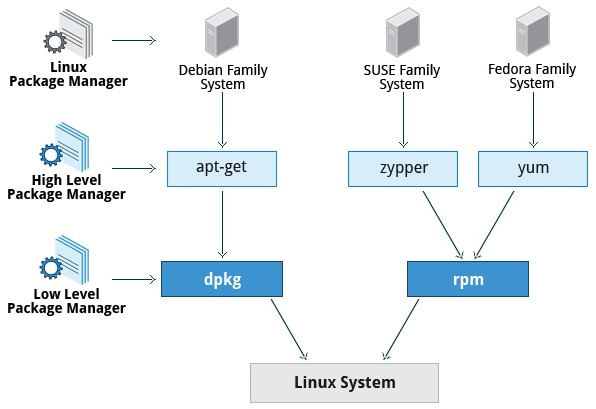
\includegraphics[width=10.5cm]{c6_soft_manager_10.jpg}
  \end{figure}
\end{frame}

\section{二进制软件包管理}
\begin{frame}
  \frametitle{二进制软件包管理 | 二进制软件包}
  \begin{block}{预编译软件包}
    预编译软件包是某个项目或程序立即可用的软件。\\
    包中通常含有可执行文件、配置示例或基本的配置、文档和辅助数据文件。\\
    包中还包含了元数据,如包的简要描述、谁或在何处编译了它、它提供了什么、它依赖于哪些包。
  \end{block}
\end{frame}

\begin{frame}
  \frametitle{二进制软件包管理 | 管理工具}
  \begin{block}{软件包管理工具}
  管理工具用于安装软件、自动安装必须预备的包、显示已安装的包、列出可用的包、显示文件列表、删除包、检索包、验证已安装的文件、提供包安全提示器等。
  \begin{itemize}
    \item 低级工具:能在后端实际安装、升级、卸载软件包文件
    \item 高级工具:负责确保能很好的执行依赖性解决和元数据检索的任务
  \end{itemize}
  \end{block}
  \pause
  \begin{table}
    \centering
    \rowcolors[]{1}{blue!20}{blue!10}
    \begin{tabularx}{0.658\textwidth}{ccc}
      \hline
      \rowcolor{blue!50}发行版 & 低级工具 & 高级工具\\
      \hline
      Debian版 & dpkg & apt/apt-get/Aptitude\\
      CentOS版 & RPM & Yum\\
      openSUSE版 & RPM & Zypper\\
      \hline
    \end{tabularx}
  \end{table}
\end{frame}

\begin{frame}
  \frametitle{二进制软件包管理 | 管理工具 | 低级 vs. 高级}
  \begin{block}{dpkg}
    基于Debian系统的一个低级包管理器。它可以安装,删除,提供有关资料,以及建立*.deb包,但它不能自动下载并安装它们相应的依赖包。
  \end{block}
  \pause
  \begin{block}{apt/apt-get}
    Debian及其衍生版的高级包管理器,并提供命令行方式来从多个来源检索和安装软件包,其中包括解决依赖性。和dpkg不同的是,apt-get不是直接基于.deb文件工作,而是基于软件包的正确名称。
  \end{block}
  \pause
  \begin{block}{Aptitude}
    基于Debian系统的另一个高级包管理器,它可用于快速简便得执行管理任务(安装,升级和删除软件包,还可以自动处理解决依赖性)。它在atp-get的基础上提供了更多功能,例如提供对软件包的几个版本的访问。
  \end{block}
\end{frame}

\begin{frame}
  \frametitle{二进制软件包管理 | 管理工具 | 低级 vs. 高级}
  \begin{block}{RPM}
    Linux标准基础(LSB)兼容发行版所使用的一种软件包管理器,用来对软件包进行低级处理。就像dpkg一样,RPM可以查询、安装、检验、升级和卸载软件包,它多数用于基于Fedora的系统,比如RHEL和CentOS。
  \end{block}
  \pause
  \begin{block}{Yum}
    相对于基于RPM的系统,Yum增加了系统自动更新的功能和带依赖性管理的软件包管理功能。作为一个高级工具,和apt-get或者Aptitude相似,Yum需要配合仓库工作。
  \end{block}
\end{frame}

\subsection{dpkg与APT包管理}
\begin{frame}
  \frametitle{二进制软件包管理 | dpkg与APT | 简介}
  \begin{block}{dpkg}
  dpkg(Debian Package)是Debian软件包管理器的基础,它被伊恩·默多克创建于1993年。dpkg与RPM十分相似,同样被用于安装、卸载和提供与 .deb软件包相关的信息。\\ 

  dpkg本身是一个底层的工具。上层的工具,像是APT,被用于从远程获取软件包以及处理复杂的软件包关系。
  \end{block}
  \pause
  \begin{block}{APT}
  APT(Advanced Packaging Tools,高级包装工具)是Debian及其派生发行版的软件包管理器。APT可以自动下载,配置,安装二进制或者源代码格式的软件包,因此简化了Linux系统上管理软件的过程。\\
  APT最早被设计成dpkg的前端,用来处理deb格式的软件包。现在经过APT-RPM组织修改,APT已经可以安装在支持RPM包管理的系统上了。
  \end{block}
\end{frame}

\begin{frame}
  \frametitle{二进制软件包管理 | dpkg与APT | \alert{dpkg}}
  \begin{table}
    \centering
    \rowcolors[]{1}{blue!20}{blue!10}
    \begin{tabularx}{\textwidth}{ccX}
      \hline
      \rowcolor{blue!50}命令 & 助记 & 作用\\
      \hline
      dpkg -c debfile & Contents & 列出软件包的内容\\
      dpkg -i debfile & Install & 安装.deb软件包\\
      dpkg -I debfile & Info & 从.deb文件中提取软件包信息\\
      dpkg -l pattern & List & 列出所有与模式相匹配的软件包\\
      dpkg -L package & Listfiles & 列出已安装软件包的文件清单\\
      dpkg -r package & Remove & 卸载已安装的软件包\\
      dpkg -P package & Purge & 完全卸载包(卸载并删除配置文件)\\
      dpkg -s package & Status & 显示已安装包的信息\\
      dpkg -S filename & Search & 查询系统中某个文件属于那个软件包\\
      \hline
    \end{tabularx}
  \end{table}
\end{frame}

\begin{frame}[fragile]
  \frametitle{二进制软件包管理 | dpkg与APT | dpkg}
  \begin{table}
    \centering
    \rowcolors[]{1}{blue!20}{blue!10}
    \begin{tabularx}{\textwidth}{cX}
      \hline
      \rowcolor{blue!50}命令 & 作用\\
      \hline
      dpkg-reconfigure package & 重新配置已安装的软件包\\
      dpkg -\!-get-selections & 获取软件包状态\\
      dpkg -\!-set-selections & 设置软件包状态\\
      dpkg -\!-force-all -\!-purge package & 强制卸载(有风险!)\\
      \hline
    \end{tabularx}
  \end{table}
\end{frame}

\begin{frame}
  \frametitle{二进制软件包管理 | dpkg与APT | dpkg}
  \begin{figure}
    \centering
    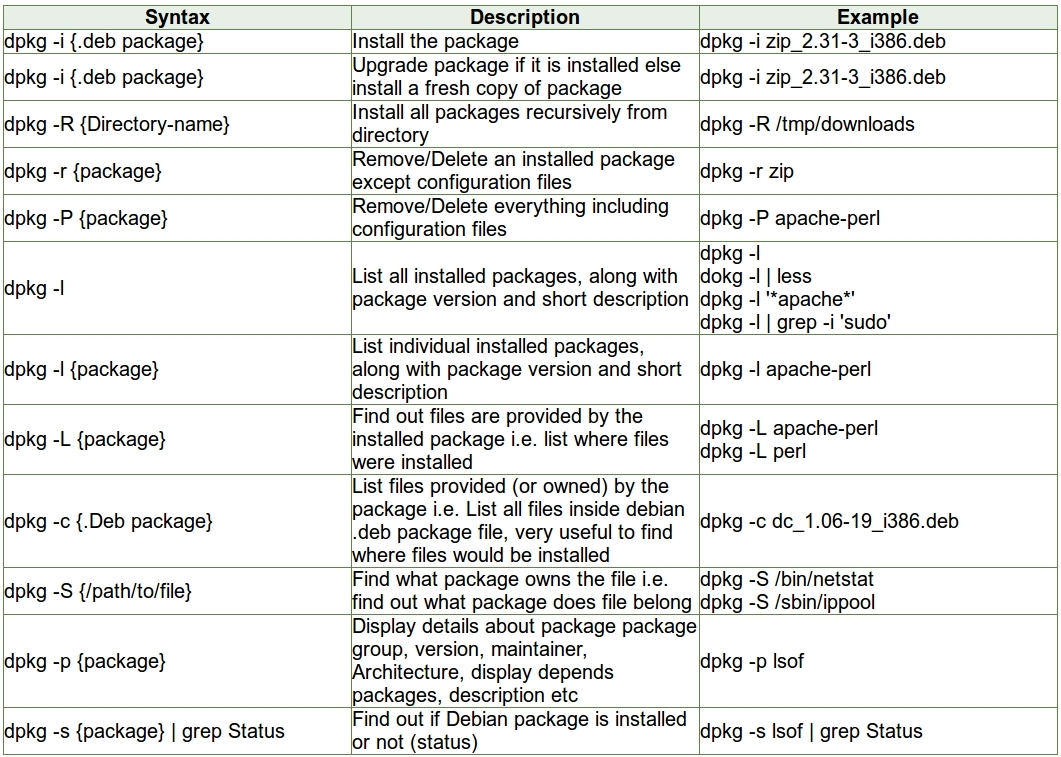
\includegraphics[width=12cm,height=8cm]{c6_dpkg_01.png}
  \end{figure}
\end{frame}

\begin{frame}
  \frametitle{二进制软件包管理 | dpkg与APT | APT | 工具}
  \begin{description}
    \item[apt/apt-get] 负责软件包的在线安装与升级,底层对deb包的处理还是用的dpkg,解决依赖关系
    \item[apt-cache] 用来查询软件包的状态和依赖关系
    \item[apt-file] 负责查询软件包名称和软件包包含的文件(值得注意的是它要自己同步)
    \item[apt-cross] 负责为交叉编译的软件包的安装与编译等
    \item[apt-offline] 可以离线安装软件包
    \item[apt-build] 可以简化源代码编译
    \item[\ldots] \ldots
  \end{description}
\end{frame}

\begin{frame}
  \frametitle{二进制软件包管理 | dpkg与APT | APT}
  \begin{table}
    \centering
    \rowcolors[]{1}{blue!20}{blue!10}
    \begin{tabularx}{\textwidth}{cX}
      \hline
      \rowcolor{blue!50}命令 & 作用\\
      \hline
      apt-cache stats & 显示软件包的统计信息\\
      apt-cache search pattern & 查找与模式相匹配的软件包\\
      apt-cache show package & 显示软件包的详细信息\\
      apt-cache depends package & 查找软件包的依赖关系\\
      apt-cache showsrc & 查看源码包的文件信息\\
      apt-cache showpkg package & 显示软件包的详细信息(包括和其他软件包的关系)\\
      \hline
    \end{tabularx}
  \end{table}
\end{frame}

\begin{frame}[fragile]
  \frametitle{二进制软件包管理 | dpkg与APT | \alert{APT}}
  \begin{table}
    \centering
    \rowcolors[]{1}{blue!20}{blue!10}
    \begin{tabularx}{\textwidth}{cX}
      \hline
      \rowcolor{blue!50}命令 & 作用\\
      \hline
      apt-get install package & 安装软件包\\
      apt-get -\!-reinstall install package & 重新安装软件包\\
      apt-get remove package & 卸载软件包(保留配置文件)\\
      apt-get -\!-purge remove package & 完全卸载软件包(删除配置文件)\\
      apt-get -f install & 修正依赖关系损坏的软件包\\
      apt-get check & 检查是否有损坏的依赖\\
      apt-get clean & 清除软件包缓存\\
      apt-get autoclean & 清除旧版本的软件包缓存\\
      apt-get autoremove & 删除不再使用的孤立软件\\
      \hline
    \end{tabularx}
  \end{table}
\end{frame}

\begin{frame}[fragile]
  \frametitle{二进制软件包管理 | dpkg与APT | \alert{APT(续)}}
  \begin{table}
    \centering
    \rowcolors[]{1}{blue!20}{blue!10}
    \begin{tabularx}{\textwidth}{cX}
      \hline
      \rowcolor{blue!50}命令 & 作用\\
      \hline
      apt-get update & 更新软件包列表\\
      apt-get upgrade & 更新已安装的软件包\\
      apt-get dist-upgrade & 升级系统到最新版本\\
      apt-get source & 下载源码包\\
      apt-get build-dep package & 构建源码包的编译环境\\
      \hline
    \end{tabularx}
  \end{table}
\end{frame}

\begin{frame}
  \frametitle{二进制软件包管理 | dpkg与APT | APT}
  \begin{figure}
    \centering
    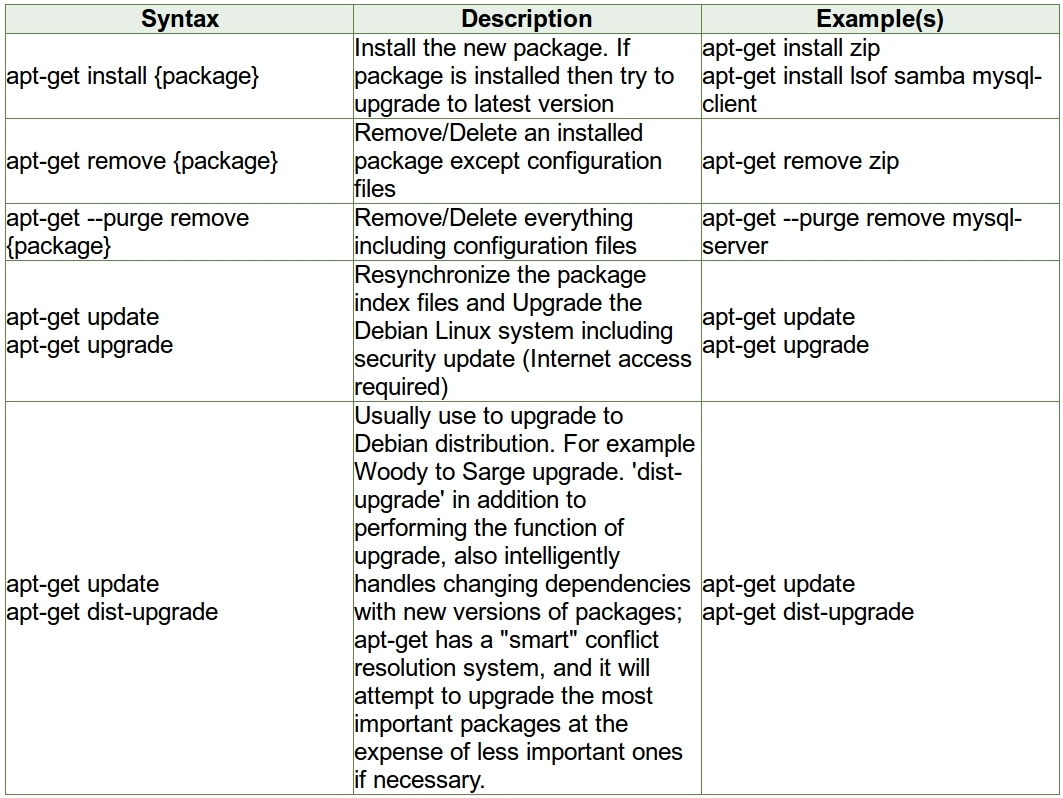
\includegraphics[width=12cm,height=8cm]{c6_apt_01.png}
  \end{figure}
\end{frame}

\begin{frame}
  \frametitle{二进制软件包管理 | dpkg与APT | Aptitude}
  \begin{block}{Aptitude}
    一个基于Ncurses的APT文字接口前端程序,是Debian及其派生系统中功能极其强大的软件包管理系统。\\
     \vspace{5pt}
    以交互形式运行时,它可以显示出所有可用的软件包,并允许用户选择包来安装或卸载。它还有一个强大的搜索系统,可通过多种搜索模式进行搜索。\\
     \vspace{5pt}
    最初,它是为Debian所开发,但现在已有可用于RPM包管理系统的派生。
  \end{block}
\end{frame}

\begin{frame}
  \frametitle{二进制软件包管理 | dpkg与APT | 比较}
  \begin{itemize}
    \item dpkg是底层工具
    \item APT是dpkg的前端
    \item Aptitude是APT的前端(字符终端)
    \item Synaptic(新立得)是APT的前端(图形界面)
  \end{itemize}
\end{frame}

\begin{frame}
  \frametitle{二进制软件包管理 | dpkg与APT | 比较}
  \begin{block}{dpkg}
    主要是对本地的软件包(本地安装的软件包和已经下载但还没有安装的deb文件)进行管理,不解决依赖关系。
  \end{block}
  \pause
  \begin{block}{APT}
    高级的软件包管理工具,在安装软件时,会自动解决软件安装过程中的依赖关系,但不会自动删除不需要的软件包。
  \end{block}
  \pause
  \begin{block}{Aptitude}
    带有UI界面的更高级的软件包管理工具,自动解决软件包安装中的依赖关系;并且在删除的时候,会自动删除不需要的软件依赖关系安装包;更加的智能、高效。有两种基本的使用方法:文本界面和命令行。
  \end{block}
\end{frame}

\begin{frame}
  \frametitle{二进制软件包管理 | dpkg与APT | \textcolor{gray}{PPA} | 简介}
  \begin{block}{PPA(Personal Package Archive,个人软件包档案)}
     因为安全或不稳定或其他种种因素,Ubuntu软件源中不可能收录所有软件,于是有了PPA,它的作用类似于Ubuntu官方的源,只不过是由个人提供打包,当然也会有某些官方源中的软件通过PPA发布不稳定版本等。\\
     \vspace{5pt}
     Ubuntu Launchpad网站提供的一项服务,当然不仅限于Launchpad。它允许个人用户上传软件源代码,通过Launchpad进行编译并发布为二进制软件包,作为APT/新立得源供其他用户下载和更新。在Launchpad网站上的每一个用户和团队都可以拥有一个或多个PPA。\\
     \vspace{5pt}
     通常PPA源里的软件是官方源里没有的,或者是最新版本的软件。相对于通过Deb包安装来说,使用PPA的好处是,一旦软件有更新,通过sudo apt-get upgrade这样命令就可以直接升级到新版本。
  \end{block}
\end{frame}

\begin{frame}
  \frametitle{二进制软件包管理 | dpkg与APT | \textcolor{gray}{PPA} | 使用}
  \begin{block}{三步走}
    \begin{enumerate}
      \item 添加PPA源:sudo add-apt-repository ppa:USER/PPA-NAME
      \item 更新所有源:sudo apt-get update
      \item 安装软件:sudo apt-get install PACKAGE\_NAME
    \end{enumerate}
  \end{block}
  \pause
  % \begin{block}{实例(安装Ubuntu Tweak)}
  %   \begin{enumerate}
  %     \item sudo add-apt-repository ppa:tualatrix/ppa
  %     \item sudo apt-get update
  %     \item sudo apt-get install ubuntu-tweak
  %   \end{enumerate}
  % \end{block}
  \begin{block}{实例(安装Java)}
    \begin{enumerate}
      \item sudo add-apt-repository ppa:webupd8team/java
      \item sudo apt-get update
      \item sudo apt-get install oracle-java8-installer
    \end{enumerate}
  \end{block}
\end{frame}

\subsection{RPM与Yum包管理}
\begin{frame}
  \frametitle{二进制软件包管理 | RPM与Yum | 简介}
  \begin{block}{RPM}
    RPM包管理器(简称RPM,全称为The RPM Package Manager)是在Linux下广泛使用的软件包管理器。最早由Red Hat研制,现在也由开源社区开发。RPM仅适用于安装用RPM来打包的软件,目前是GNU/Linux下软件包资源最丰富的软件包类型之一。\\
    RPM软件包分为二进制包(Binary)、源代码包(Source)和Delta包三种。二进制包可以直接安装在计算机中,而源代码包将会由RPM自动编译、安装。源代码包经常以src.rpm作为后缀名。
  \end{block}
  \pause
  \begin{block}{Yum}
    Yum(Yellow dog Updater, Modified)由Duke University团队,修改Yellow Dog Linux的Yellow Dog Updater开发而成,是一个基于RPM包管理的字符前端软件包管理器。能够从指定的服务器自动下载RPM包并且安装,可以处理依赖性关系,并且一次安装所有依赖的软件包,无须繁琐地一次次下载、安装。
  \end{block}
\end{frame}

\begin{frame}
  \frametitle{二进制软件包管理 | RPM与Yum | RPM | 功能}
  \begin{table}
    \centering
    \rowcolors[]{1}{blue!20}{blue!10}
    \begin{tabularx}{0.6\textwidth}{ccX}
      \hline
      \rowcolor{blue!50}选项 & 助记 & 说明\\
      \hline
      -q & Query & 查询软件包\\
      -V & Verify & 校验软件包\\
      -i & Install & 安装软件包\\
      -e & Erase & 删除软件包\\
      -U & Upgrade & 升级软件包 \\
      \hline
    \end{tabularx}
  \end{table}
\end{frame}

\begin{frame}
  \frametitle{二进制软件包管理 | RPM与Yum | RPM | 选项}
  \begin{table}
    \centering
    \rowcolors[]{1}{blue!20}{blue!10}
    \begin{tabularx}{\textwidth}{cclX}
      \hline
      \rowcolor{blue!50}选项 & 助记 & 说明 & 类别\\
      \hline
      -v & Verbose & 详细信息 & 通用选项\\
      \hline
      -a & All & 所有已安装的软件包 & 选择选项\\
      -f & File & 文件所属软件包 & \\
      -p & Package & 指定软件包(.rpm) & \\
      \hline
    \end{tabularx}
  \end{table}
\end{frame}

\begin{frame}[fragile]
  \frametitle{二进制软件包管理 | RPM与Yum | RPM | 选项}
  \begin{table}
    \centering
    \rowcolors[]{1}{blue!20}{blue!10}
    \begin{tabularx}{\textwidth}{cclX}
      \hline
      \rowcolor{blue!50}选项 & 助记 & 说明 & 类别\\
      \hline
      -l & List & 软件包中的文件列表 & 查询选项\\
      -i & Info & 软件包的信息 & \\
      -c & Configfiles & 配置文件 & \\
      -d & Docfiles & 文档文件 & \\
      -R & Requires & 软件包依赖关系 & \\
      -s & State & 软件包状态 & \\
      \hline
      -h & Hash & 进度条 & 安装选项\\
      -\!-nodeps & --- & 不检查依赖性 & \\
      -\!-excludedocs & --- & 不安装文档 & \\
      -\!-prefix & --- & 指定安装路径 & \\
      -\!-test & --- & 测试而不安装 & \\
      -\!-replacepkgs & --- & 覆盖安装 & \\
      -\!-replacefiles & --- & 替换文件 & \\
      -\!-force & --- & 强制安装 & \\
      \hline
    \end{tabularx}
  \end{table}
\end{frame}

\begin{frame}
  \frametitle{二进制软件包管理 | RPM与Yum | RPM | \alert{命令}}
  \begin{table}
    \centering
    \rowcolors[]{1}{blue!20}{blue!10}
    \begin{tabularx}{\textwidth}{cX}
      \hline
      \rowcolor{blue!50}命令 & 作用\\
      \hline
      rpm -qa & 查询系统中已经安装的软件包\\
      rpm -qf file & 查询已安装的文件属于那个软件包\\
      rpm -ql package & 查询已安装软件包把文件安装到何处\\
      rpm -qi package & 查询已安装软件包的信息\\
      rpm -qc package & 查询已安装软件包的配置文件\\
      rpm -qd package & 查询已安装软件包的文档文件\\
      rpm -qR package & 查询已安装软件包的依赖关系\\
      \hline
      rpm -qpi rpmfile & 查询软件包的信息\\
      rpm -qpl rpmfile & 查询软件包的文件列表\\
      rpm -qpd rpmfile & 查询软件包的文档文件\\
      rpm -qpc rpmfile & 查询软件包的配置文件\\
      rpm -qpR rpmfile & 查询软件包的依赖关系\\
      \hline
      rpm -ivh rpmfile & 安装软件包\\
      rpm -Uvh rpmfile & 升级软件包\\
      rpm -e package & 删除软件包\\
      \hline
    \end{tabularx}
  \end{table}
\end{frame}

\begin{frame}
  \frametitle{二进制软件包管理 | RPM与Yum | RPM}
  \begin{figure}
    \centering
    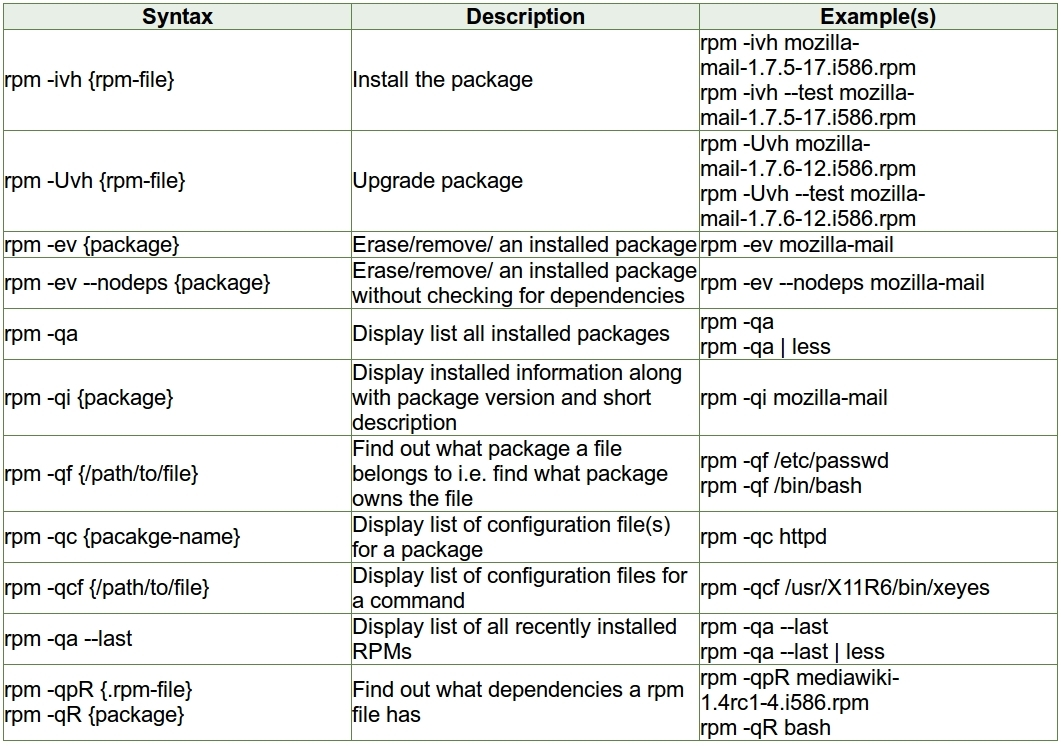
\includegraphics[width=12cm,height=8cm]{c6_rpm_01.png}
  \end{figure}
\end{frame}

\begin{frame}
  \frametitle{二进制软件包管理 | RPM与Yum | \alert{Yum}}
  \begin{table}
    \centering
    \rowcolors[]{1}{blue!20}{blue!10}
    \begin{tabularx}{\textwidth}{cX}
      \hline
      \rowcolor{blue!50}命令 & 作用\\
      \hline
      yum install package & 安装软件包\\
      yum remove package & 删除软件包\\
      yum check-update & 检查可以更新的软件包\\
      yum update & 更新所有软件包\\
      yum update package & 更新指定软件包\\
      yum upgrade & 升级系统\\
      yum clean package & 清除缓存中的rpm软件包\\
      \hline
      yum list & 列出所有可以安装或更新的软件包\\
      yum list package & 列出指定的软件包\\
      yum list updates & 列出所有可以更新的软件包\\
      yum list installed & 列出所有已经安装的软件包\\
      yum info & 列出所有可以安装或更新的软件包的信息\\
      yum search pattern & 搜索匹配模式的软件包\\
      yum provides file & 搜索包含指定文件的软件包\\
      \hline
    \end{tabularx}
  \end{table}
\end{frame}

\begin{frame}
  \frametitle{二进制软件包管理 | RPM与Yum | Yum}
  \begin{figure}
    \centering
    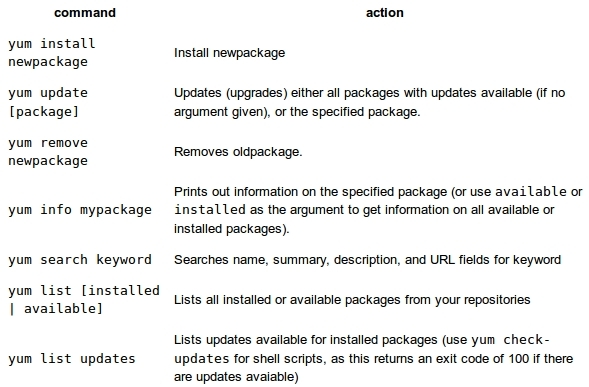
\includegraphics[width=11cm]{c6_yum_01.png}
  \end{figure}
\end{frame}

\subsection{二进制软件包管理比较}
\begin{frame}
  \frametitle{二进制软件包管理 | 比较}
  \begin{figure}
    \centering
    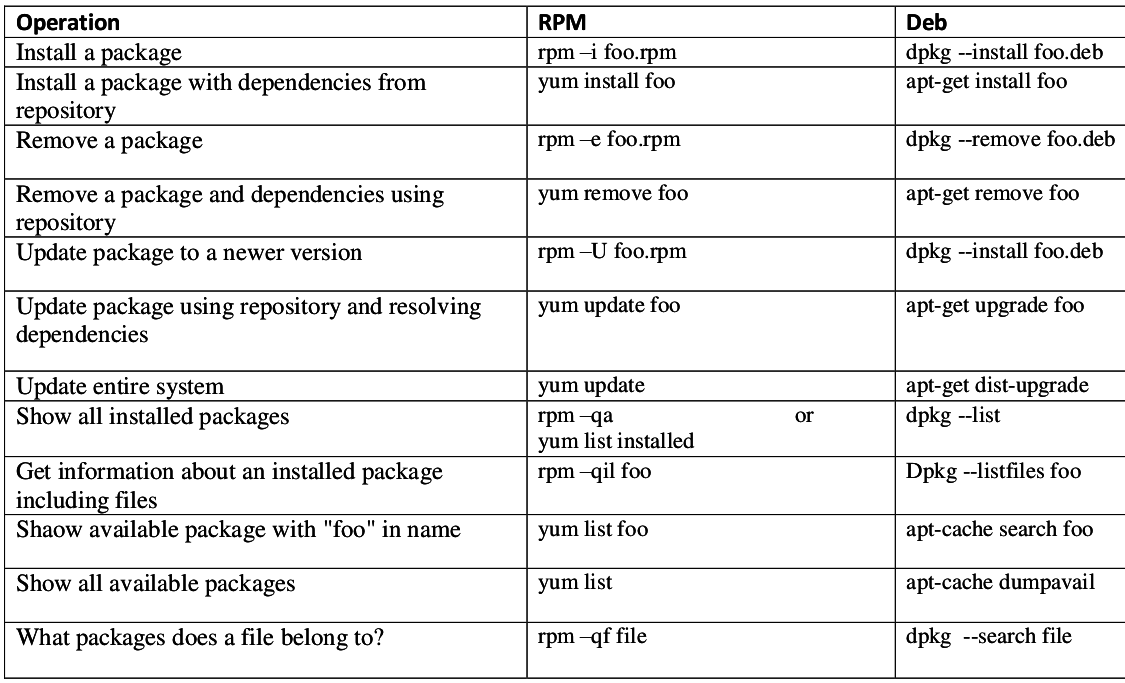
\includegraphics[width=12cm]{c6_apt_yum_02.png}
  \end{figure}
\end{frame}

\begin{frame}
  \frametitle{二进制软件包管理 | 比较}
  \begin{figure}
    \centering
    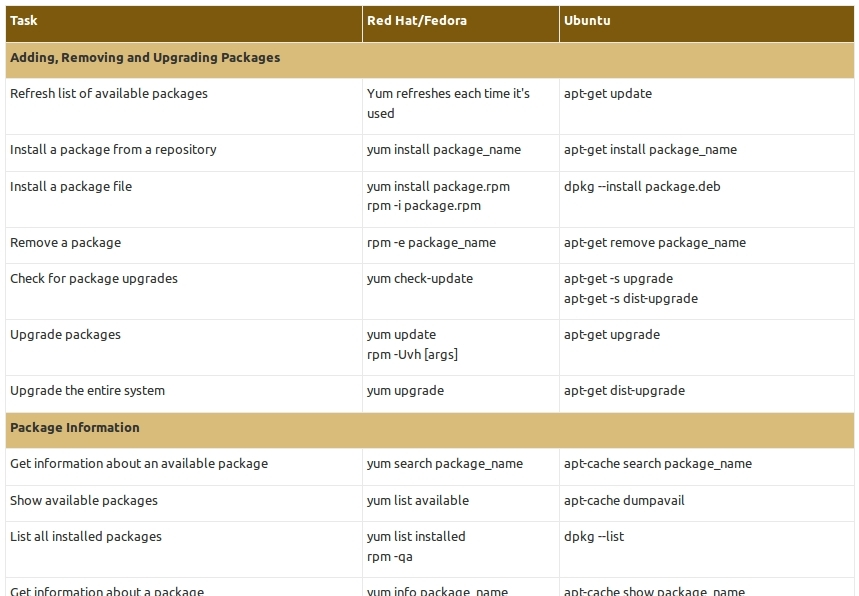
\includegraphics[width=12cm,height=8cm]{c6_apt_yum_01.png}
  \end{figure}
\end{frame}

\begin{frame}
  \frametitle{二进制软件包管理 | 比较}
  \begin{figure}
    \centering
    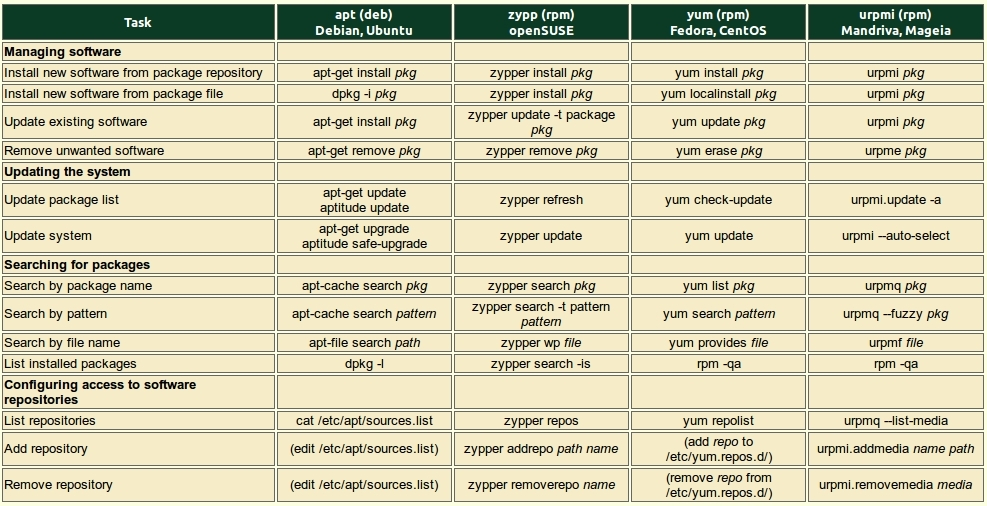
\includegraphics[width=12cm]{c6_compare_all_01.png}
  \end{figure}
\end{frame}

\begin{frame}
  \frametitle{二进制软件包管理 | 比较}
  \begin{figure}
    \centering
    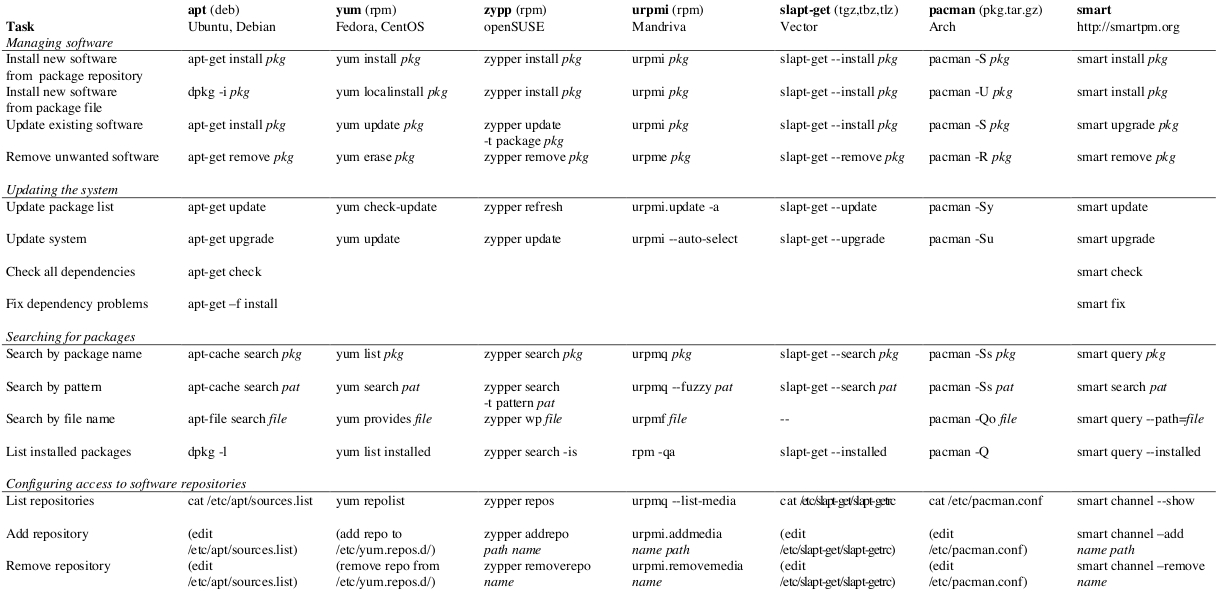
\includegraphics[width=12cm]{c6_compare_all_02.png}
  \end{figure}
\end{frame}

\section{源代码安装}
\subsection{源代码}
\begin{frame}
  \frametitle{源代码安装 | 源代码}
  \begin{block}{源代码}
    源代码是创建软件的原始数据。\\
    下载的源代码包通常提供由C、C++、Perl、Python或其他编程语言编写的源代码和文档,其中包括编译说明、帮助编译和安装软件的脚本和实用工具、数据文件、配置示例和各种其他文件。
  \end{block}
\end{frame}

\subsection{开放源代码许可证}
\begin{frame}
  \frametitle{源代码安装 | 开放源代码}
  \begin{block}{开放源代码}
    以源代码形式提供的软件通常称为开放源代码(open source)。\\
    开放源代码软件是带有特定许可条款的软件,通常可以自由地查看、共享和使用它,(最重要的是)还可以自由地修改它。
  \end{block}
  \pause
  \begin{block}{开放源代码许可证}
    开放源代码软件许可证声明对源代码拥有版权,并确定代码的使用和发布、以及派生代码的使用和发布的自由范围和限制。
  \end{block}
\end{frame}

\begin{frame}
  \frametitle{源代码安装 | 开源许可证}
  \begin{figure}
    \centering
    
\includegraphics[width=10cm]{c6_license_01.png}
  \end{figure}
\end{frame}

\begin{frame}
  \frametitle{源代码安装 | 开源许可证 | BSD}
  \begin{block}{BSD许可证}
    \alert{BSD}许可证(Berkeley Software Distribution license),是自由软件中使用最广泛的许可证之一。BSD(Berkeley Software Distribution,伯克利软件套件,Unix变种)就是遵照这个许可证来发布的,该许可证也因此而得名。\\
    跟其他许可证相比,从GNU通用公共许可证(GPL)到限制重重的著作权(Copyright),BSD许可证比较宽松,甚至跟公有领域更为接近。事实上,BSD许可证被认为是copycenter(中间版权),界乎标准的copyright与GPL的copyleft之间。GPL强迫后续版本必须一样是自由软件,BSD的后续版本可以选择要继续是BSD或其他自由软件条款或封闭软件等等。\\
    遵守BSD许可证的软件,允许用作商业用途,甚至可按照专属许可证进行再发布。比较著名的例子如微软产品中引入了BSD网络部分的代码,Mac OS X中使用了不少FreeBSD的组件。也可以将一部分遵照BSD许可证发布,另外一些采取其他许可证。
  \end{block}
\end{frame}

\begin{frame}
  \frametitle{源代码安装 | 开源许可证 | GPL}
  \begin{block}{GPL}
    GNU通用公共许可协议(GNU General Public License,缩写:GNU GPL、GPL),是一个广泛被使用的自由软件许可协议条款,最初由理查德·斯托曼(Richard Matthrew Stallman)为GNU计划而撰写。\\
    \vspace{0.5em}
    \alert{GPL} 给予了计算机程序自由软件(free software)的定义,并且使用Copyleft来确保程序的自由被完善的保留。\\
    \vspace{0.5em}
GPL与其他一些更“许可的”自由软件许可证(比如BSD许可证)相比,主要区别就在于GPL寻求确保“自由”能在复制件及演绎作品中得到保障。它通过一种由斯托曼发明的叫Copyleft的法律机制实现,即要求GPL程序的演绎作品也要在GPL之下。相反,BSD式的许可证并不禁止演绎作品变成专有软件。
  \end{block}
\end{frame}

\begin{frame}
  \frametitle{源代码安装 | 开源许可证 | GPL}
  \begin{block}{“自由”:free speech vs. free beer}
    GPL授予程序接受人以下权利,或称“自由”:以任何目的运行此程序的自由;再发行复制件的自由;改进此程序,并公开发布改进的自由(前提是能得到源代码)。
  \end{block}
  \pause
  \begin{block}{\alert{“自由”}}
    \begin{itemize}
      \item 使用的自由:可以不受任何限制地使用软件
      \item 研究的自由:可以获得软件源代码、研究软件运作方式
      \item 散布的自由:可以自由复制软件及散布给他人
      \item 改良的自由:可以自行改良软件并散布改良后的版本
    \end{itemize}
  \end{block}
  \pause
  \begin{block}{“病毒”}
    GPL条款规定演绎作品也必须是GPL的:对已发布的软件所作的任何修改都必须以相同的许可证发布。
  \end{block}
\end{frame}

\begin{frame}
  \frametitle{源代码安装 | 开源许可证 | GPL}
  \begin{enumerate}
    \item The freedom to use the software for any purpose.
    \item The freedom to change the software to suit your needs.
    \item The freedom to share the software with your friends and neighbors.
    \item The freedom to share the changes you make.
  \end{enumerate}
\end{frame}

\begin{frame}
  \frametitle{源代码安装 | 开源许可证 | GPL}
  \begin{figure}
    \centering
    
\includegraphics[width=10cm]{c6_copy_03.jpg}
  \end{figure}
\end{frame}

\begin{frame}
  \frametitle{源代码安装 | 开源许可证 | 选择}
  \begin{figure}
    \centering
    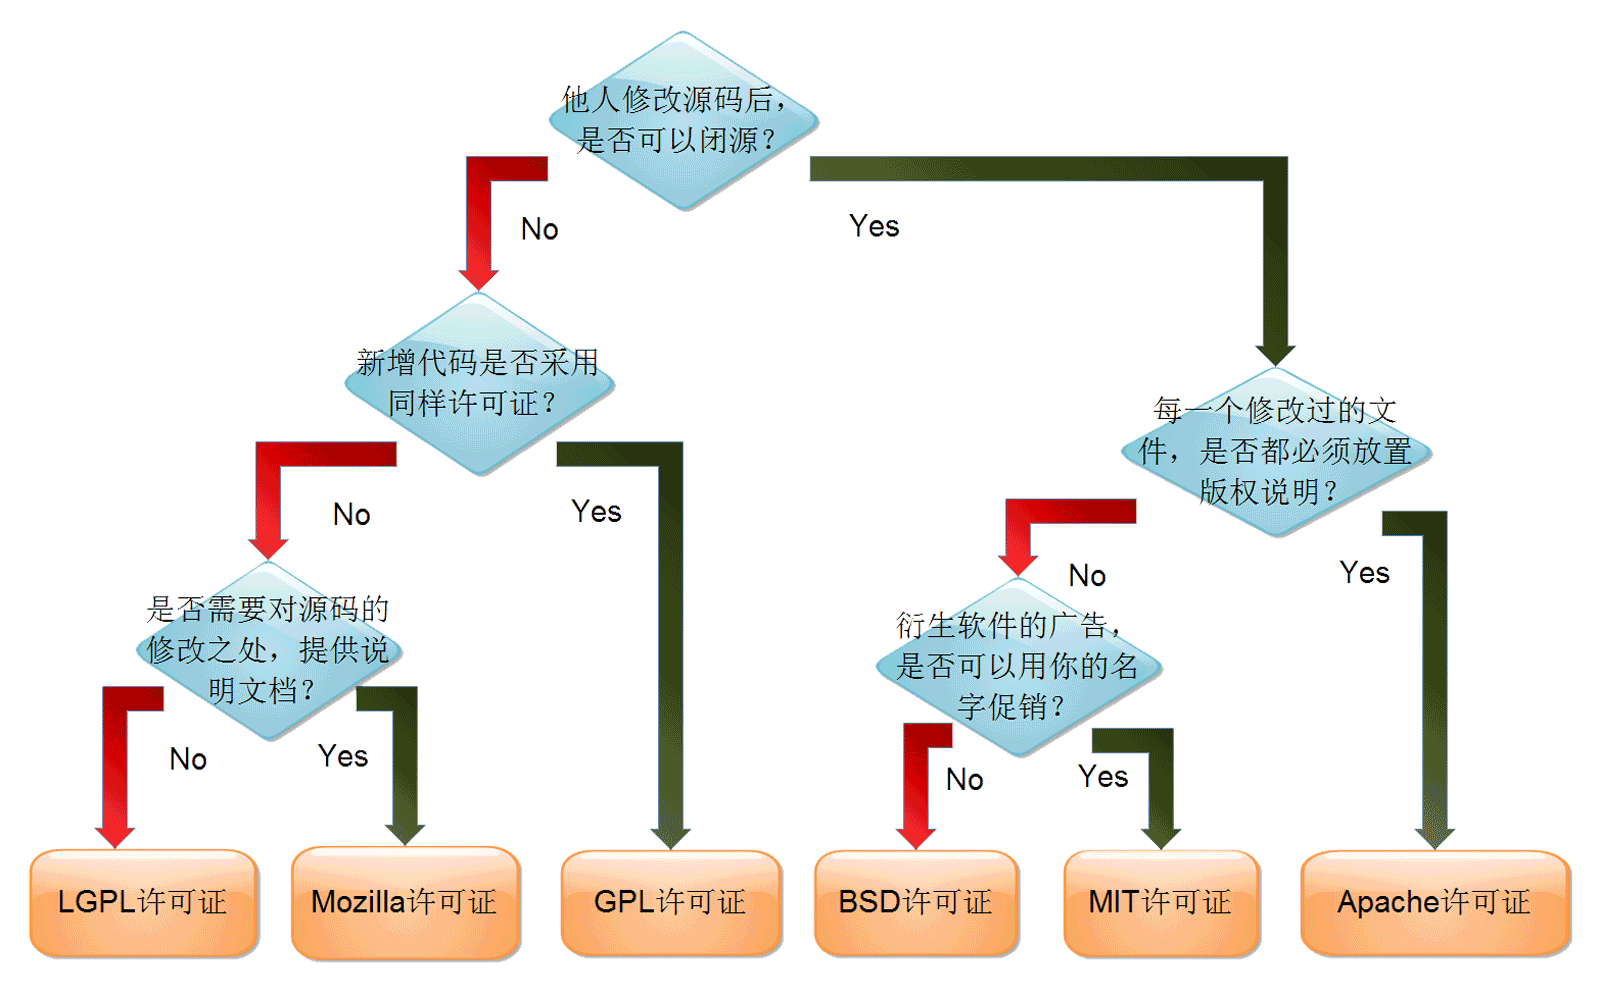
\includegraphics[width=11cm]{c6_license_choose_01.png}
  \end{figure}
\end{frame}

\subsection{选择软件}
\begin{frame}
  \frametitle{源代码安装 | 选择软件}
  \begin{itemize}
    \item 最新的正式版本\\
      一般以“LATEST”进行标记,通常情况下应该下载、安装正式版本。
    \item 在多个平台上稳定运行的以前的版本
    \item 用于测试的开发版本\\
      测试版本通常称为alpha、beta、候选版本(RC,release candidate)或每日快照(daily snapshot),它是潜在不稳定的,使用时必须小心。
  \end{itemize}
\end{frame}

\subsection{下载软件}
\begin{frame}
  \frametitle{源代码安装 | 下载软件}
  \begin{block}{文件格式}
    下载的源代码文件内容通常由tar、gzip、bzip命令打包压缩过,形成的文件称为tarball,其典型的文件扩展名是 .tgz、.tar.gz或 .tar.bz2。
  \end{block}
  \pause
  \begin{block}{下载技巧}
    \begin{itemize}
      \item Web浏览器:Firefox,Chrome
      \item FTP客户端:FileZilla
      \item 命令行:wget,lftp,curl
    \end{itemize}
  \end{block}
  \pause
  \begin{block}{文件校验}
    \begin{itemize}
      \item md5:md5sum,md5deep
      \item SHA1:sha1sum,sha1deep
      \item SHA256:sha256sum,sha256deep
      \item CRC-32:crc32
    \end{itemize}
  \end{block}
\end{frame}

\subsection{编译和安装}
\begin{frame}[fragile]
  \frametitle{源代码安装 | \alert{编译和安装}}
  \begin{block}{准备工作}
    \begin{enumerate}
      \item 下载软件:\verb|wget -c https://url/software.tar.gz|
      \item 提取文件:\verb|tar -xzvf software.tar.gz|
      \item 切换目录:\verb|cd software|
    \end{enumerate}
  \end{block}
  \pause
  \begin{block}{安装软件}
    \begin{enumerate}
      \item 配置环境:\verb|./configure| (分析程序构建环境)
      \item 编译软件:\verb|make| (只构建需要构建的内容)
      \item 安装软件:\verb|make install|
    \end{enumerate}
  \end{block}
\end{frame}

\begin{frame}[fragile]
  \frametitle{源代码安装 | 编译和安装}
  \begin{block}{补充说明}
    \begin{itemize}
      \item 阅读软件的指南或说明:\verb|vim INSTALL|,或 \verb|vim README|
      \item 指定软件的安装目录:\verb|./configure --prefix=PATH|
      \item 安装软件前进行测试:\verb|make test|,或 \verb|make check|
      \item 以超级用户身份安装软件:\verb|sudo make install|
      \item 删除编译产生的临时文件:\verb|make clean|
    \end{itemize}
  \end{block}
\end{frame}

\begin{frame}
  \frametitle{源代码安装 | 编译和安装}
  \begin{figure}
    \centering
    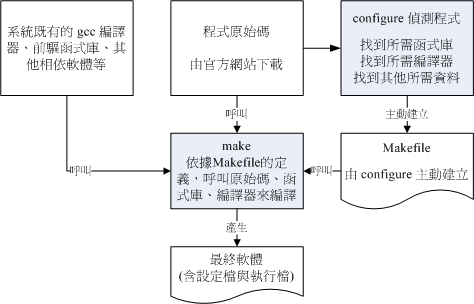
\includegraphics[width=9cm]{c6_make_01.png}
  \end{figure}
\end{frame}

\section{脚本安装}
\begin{frame}[fragile]
  \frametitle{脚本安装 | \alert{基本步骤}}
  \begin{block}{基本步骤}
    \begin{enumerate}
      \item 下载软件:\verb|wget -c https://url/software.tar.gz|
      \item 提取文件:\verb|tar -xzvf software.tar.gz|
      \item 切换目录:\verb|cd software|
      \item 查阅说明:\verb|vim README|
      \item 安装软件:\verb|./setup.sh|,或 \verb|./install.sh|
    \end{enumerate}
  \end{block}
\end{frame}

\section{使用biocoda管理生信软件}
\begin{frame}
  \frametitle{biocoda | conda | 简介}
  \begin{block}{conda}
    Conda是开源的包管理系统和环境管理系统,可以安装软件包的多个版本和依赖,而且各环境之间可以很方便得切换。Conda支持Linux,Mac OS X和Windows系统。\\
    \vspace{0.5em}
    Conda主要为Python程序所创建,但是可以打包和分布任意软件。\\
    Package, dependency and environment management for any language—Python, R, Ruby, Lua, Scala, Java, JavaScript, C/ C++, FORTRAN.\\
    \vspace{0.5em}
    Conda有多个版本,包括Anaconda, Anaconda Server和Miniconda。
  \end{block}
\end{frame}

\begin{frame}[fragile]
  \frametitle{biocoda | conda | 安装配置}
  \begin{block}{安装与配置}
    \begin{enumerate}
      \item 下载\\ \verb|wget -c https://url/Miniconda3-latest-Linux-x86_64.sh|
      \item 安装\\ \verb|bash Miniconda3-latest-Linux-x86_64.sh|
      \item 配置(修改 .bashrc)\\ \verb|export PATH="PathToMiniconda/bin:$PATH"|
      \item 配置 .bashrc(修改 .profile)\\ \verb|source $HOME/.bashrc|
    \end{enumerate}
  \end{block}
\end{frame}

\begin{frame}
  \frametitle{biocoda | 简介}
  \begin{block}{biocoda}
    Bioconda is a channel for the conda package manager specializing in bioinformatics software. Bioconda consists of:
    \begin{itemize}
      \item a repository of recipes hosted on GitHub
      \item a build system that turns these recipes into conda packages
      \item a repository of >1500 bioinformatics packages ready to use with conda install
      \item Over 130 contributors that add, modify, update and maintain the recipes
    \end{itemize}
  \end{block}
\end{frame}

\begin{frame}[fragile]
  \frametitle{biocoda | 使用}
  \begin{block}{Using biocoda}
    Bioconda supports only 64-bit Linux and Mac OSX.
    \begin{enumerate}
      \item Install conda
      \item Set up channels (It is important to add them in this order)
\vspace{-0.5em}
\begin{lstlisting}
conda config --add channels defaults
conda config --add channels conda-forge
conda config --add channels bioconda
\end{lstlisting}
\vspace{-0.8em}
      \item Install packages
\vspace{-0.5em}
\begin{lstlisting}
# install into the current conda environment:
conda install bwa
# a new environment can be created
conda create -n aligners bwa bowtie
\end{lstlisting}
    \end{enumerate}
  \end{block}
\end{frame}

\begin{frame}[fragile]
  \frametitle{biocoda | 使用镜像加速}
  \begin{block}{镜像}
    \begin{itemize}
      \item 清华(TUNA)镜像\\ \verb|https://mirrors.tuna.tsinghua.edu.cn|
      \item 中科大(USTC)镜像\\ \verb|https://mirrors.ustc.edu.cn|
    \end{itemize}
  \end{block}
  \pause
  \begin{block}{添加镜像(1/2)}
    \begin{itemize}
      \item Anaconda
\begin{lstlisting}
conda config --add channels TUNA/anaconda/pkgs/main/
conda config --add channels TUNA/anaconda/pkgs/free/
conda config --set show_channel_urls yes
\end{lstlisting}
    \end{itemize}
  \end{block}
\end{frame}

\begin{frame}[fragile]
  \frametitle{biocoda | 使用镜像加速}
  \begin{block}{添加镜像(2/2)}
    \begin{itemize}
      \item Conda Forge
\begin{lstlisting}
conda config --add channels TUNA/anaconda/cloud/conda-forge/
\end{lstlisting}
      \item R \& biocoda
\begin{lstlisting}
conda config --add channels TUNA/anaconda/pkgs/r/
conda config --add channels TUNA/anaconda/cloud/bioconda/
\end{lstlisting}
    \end{itemize}
  \end{block}
\end{frame}

\begin{frame}
  \frametitle{biocoda | 参考资料}
  \begin{itemize}
    \item \href{https://conda.io/docs/}{conda使用手册}
    \item \href{https://bioconda.github.io/}{bioconda}
    \item \href{https://mirrors.tuna.tsinghua.edu.cn/help/anaconda/}{Anaconda镜像使用帮助}
    \item \href{https://github.com/Yixf-Education/demo4bx/tree/master/conda}{生物信息学软件的安装与维护}
  \end{itemize}
\end{frame}

\section{回顾与总结}
\subsection{总结}
\begin{frame}
  \frametitle{软件安装 | 总结}
  \begin{block}{知识点}
    \begin{itemize}
      \item 软件包管理:软件包的类型,管理系统
      \item 二进制软件包管理:dpkg与APT,RPM与Yum
      \item 源代码安装:开源许可证,版本选择,安装步骤
      \item 脚本安装:基本步骤
    \end{itemize}
  \end{block}
  \begin{block}{技能}
    \begin{itemize}
      \item Ubuntu中的软件管理
      \item CentOS中的软件管理
      \item 通过源代码安装软件
      \item 使用conda管理生信软件
    \end{itemize}
  \end{block}
\end{frame}

\subsection{思考题}
\begin{frame}
  \frametitle{软件安装 | 思考题}
  \begin{enumerate}
    \item Ubuntu和CentOS使用的软件包管理系统分别是什么?
    \item 列举dpkg和APT软件包管理中的常用命令及其作用。
    \item 列举RPM和Yum软件包管理中的常用命令及其作用。
    \item 列举几个常见的开放源代码许可证。
    \item GPL授予程序使用者哪些“自由”?
    \item 通过源代码安装软件的基本步骤是什么?
  \end{enumerate}
\end{frame}

\begin{frame}
  \frametitle{下节预告}
  你知道哪些编辑器?用过哪些编辑器?有何感受?\\
  总结编辑文件时的常见操作。你是如何完成这些操作的?
\end{frame}



\section*{Acknowledgements}
\begin{frame}
  \frametitle{Powered by}
  \begin{center}
    
\includegraphics[width=9cm]{power.png}
  \end{center}
\end{frame}

\end{document}


